\begin{savequote}[75mm] 
Nulla facilisi. In vel sem. Morbi id urna in diam dignissim feugiat. Proin molestie tortor eu velit. Aliquam erat volutpat. Nullam ultrices, diam tempus vulputate egestas, eros pede varius leo.
\qauthor{Quoteauthor Lastname} 
\end{savequote}

\chapter{Implementation}
\label{chapterfive}

This chapter provides information on how the cloudlet is implemented. Information on how to create a service for the cloudlet is also included. We also provide information about the various classes which play a vital role in the cloudlet platform.

\section{Component structure}
\label{sect:structure}

Figure \ref{fig:objstruc} shows the class hierarchy and components which make the cloudlet. The system has been segmented into numerous logical components. There is a management component, controller and communication \& event handlers. The responsibility of the controller class, as it's name suggests, is to control the ensure that various parts of the cloudlet start running at the neccessary times. It is the entry point for the system. Its responsibility is to receive a port number and start the mosquitto event handler (thus start mosquitto) and the communication handler on the specified port. The MQTT protocol is used for communication between the clients and the cloudlet. MQTT uses a publish-subscribe messaging pattern. This has the implications that it uses channels. Clients can subscribe to channels and recieve data which is published by the cloudlet on those channels. The communication handler is responsible for subscribing to the appropriate channels which are used by clients t publish data or send requests to the cloudlet. These channels allow the following actions:
\begin{itemize}
\item joining a cloudlet
\item requesting a service list
\item requesting a connected user list from the clients
\end{itemize}
The communication handler also uses the service manager and
user manager. The service manager and the user manager form the management component. Their responsibility is to keep track of connected users, avalaiable services and preform other actions related to services and users. The mosquitto event handler class is designed to extend mosquitto. It detects client connections and disconnections. The service manager is responsible for keeping track of available services, loading them and other management tasks for services. The user manager keeps track of online users and the services they are using. Cloudlet services can be physically located on the cloudlet and or the clients, and those clients can be mobile devices or laptops. Figure \ref{fig:objstruc} shows a service as being in the intersection of front-end (clients) and the back-end (cloudlet on raspberry pi).

\begin{figure}
\centering
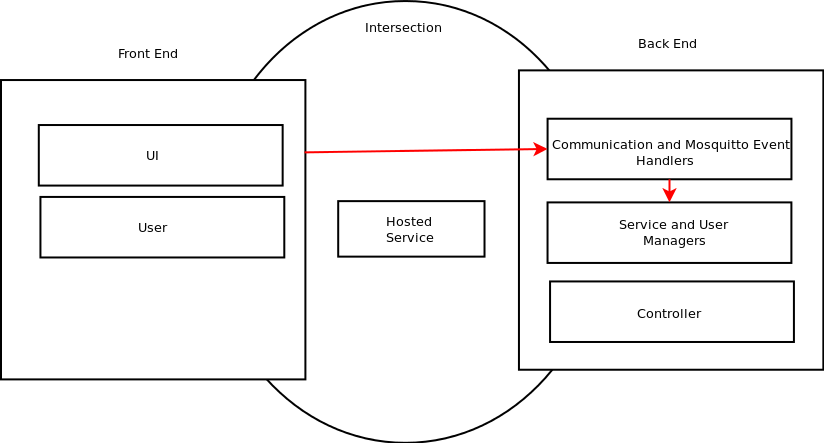
\includegraphics[scale=0.4]{figures/newcomponentstructure}
\caption{Classes that make up cloudlet. Red lines show communication between components.}
\label{fig:objstruc}
\end{figure}


\subsection{Mosquitto Event Handler}
Mosquitto, as stated above in section \ref{communication}, is an open-source broker that implements version 3.1 of the MQTT protocol. Mosquito does not have a mechanism that allows applications to hook into such that they are alerted of connections and disconnections. However, the application writes messages on the standard error stream when there is a connection or disconnection. The mosquitto event handler is a class created to make it possible to automatically capture client connections and disconnections. This is done by allowing the mosquitto event handler class to start a mosquitto process and capture it's error stream. The data on that stream is used to alert the communication handler of connections and disconnections. The readiness of the standard error stream, that is the availability of data on that stream, is determined by using the ``select" system call which is available for all Unix-like and POSIX-compliant operating systems. The cloudlet is created to cater for hosting multiple services. The design of the mosquitto event handler class takes this into account. It uses the observer pattern. This is the pattern where subscribers (services) are enabled to register with and receive notifications from a provider, the provider being mosquitto event handler class. Using this pattern makes it possible for services to register with the  mosquitto event handler class and they will receive notifications in the case where a client connects or disconnects on the cloudlet.


\subsection{Service}
The service can be located on the raspberry pi or on the phone. This is illustrated in figure \ref{fig:objstruc}. The service class contains information about a service such as it's name and description. It also handles service requests which have already been granted by the user manager and service manager. The user manager and service manager are designed to also grant or deny service requests. They have been implemented in such a manner because future releases of the cloudlet should allow the cloudlet owners to ban certain users. This functionality is not accessible with this release as ownership of the cloudlet is not within the scope of this project. The implementation of the services on the cloudlet requires communication between service and clients to not go through the communication handler. The only communication that goes through the communication handler are the actions clients can make which belong to the base cloudlet, that is, they belong to no service. These actions are listed in section \ref{sect:structure}. In the event where clients request a service, they are allocated an IP and port to connect to using TCP. This is because services cannot use the mosquitto channels for communication as channels require the payload to not exceed 260MB. The mobile device has the ability to host services therefore it can advertise hosted services. The names chosen for services need not be descriptive and because of this, each
service has a string which acts as it's metadata. The string looks as follows:

\begin{lstlisting}
``Name=somename;CloudletV=somenumber;
Description=somedescription.;authors=somename;
Copyright=Copyright someyear somename;
Website=https://example.com".
\end{lstlisting}

\noindent This information should be sufficient in the identification of service by humans. In addition, since this metadata is sent as one string. It removes the need for the client to request various fields which it needs.

\section{Client connections and actions}
The client is identified using a combination of the mac address and their chosen username. In order to join a cloudlet, the client must first connect to a WiFi access point named ``CloudletX". The client should then connect to the mqtt broker, mosquitto. The address of the broker is fixed and it is ``10.10.0.51:9999". The mqtt protocol requires clients to identify themselves and the clients should use a combination of the mac address and username. These should be formated in the form “<mac address>|<username>”, and we shall refer to this combination as the identifier. After connecting to the MQTT broker, the client should then subscribe to the following channels:

\begin{itemize}
\item client/connecteduser/<username> - All messages received on this channel are identifiers of users connected to the cloudlet.
\item client/service/<useraname> -  All messages received on this channel are identifiers of services available on the cloudlet.
\item client/serviceuserslist/<username> -  All messages received on this channel are lists of users who use a service whose name was provided when the request for the list was made.
\item server/login/<name> - This channel is used once, when the client attempts to connect to the cloudlet. The message received on this channel is the connection status.
\item client/service\_request/recvIP - This channel is used to provide clients with an ip and port to use to connect to the requested service.
\item client/service\_request/<identifier> - This channel is used for requests made by other clients for a service hosted on this client.
\end{itemize}

The cloudlet will provide the client with 2 seconds in order for it to subscribe to the channels. After which, a response will be received on the client side on the channel “server/login/<name>”. The response can either be OK , UDUP or MDUP. OK means that the client is connected. UDUP means that the client has a duplicate username is will not be connected to the cloudlet. MDUP means that the client has a duplicate mac address and will not be connected to the cloudlet as a result.\newline

The are channels used for outgoing traffic. These channels are used for the requests made by the clients to the cloudlet. These actions are the requesting of a service list, requesting a list of connected users from the cloudlet and requesting a list of users of a service. There are other actions such as advertising services and requesting a service. The following table shows the channels, the payload one must send for each action and their role.

\begin{center}
  \begin{tabular}{ l | c | l }
    \hline
    Channel & Payload & Role \\ \hline \hline
    server/serviceusers & servicename + "|" + name & Used for requesting connected to cloudlet using the specified service \\ \hline
    server/connectedusers & name & Used for requesting connected to cloudlet \\ \hline
    server/servicelist & name & Used for requesting list of available services on cloudlet \\ \hline
    server/useservice & identifier + ";" + servicename & Used to request a service. \\ \hline
    server/service  & services json string & Used to advertize services hosted on the client. \\
    \hline
  \end{tabular}
\end{center}

\section{Creating a service}

\subsection{Cloudlet}
The services and code are separated on the cloudlet. The services which reside in the cloudlet are located in the folder ``services". This makes it easy to identify and be able to remove services when necessary. In order to create a service in the cloudlet, one must create a subfolder inside ``services". The folder name should be the name of the service and have no spacing. Figure \ref{fig:folderstructure} shows the folder structure of a cloudlet with a service named ``file\_sharer". Only two files should be created in the folder that has the service name. The files are ``\_\_init\_\_.py" and ``description.txt". All service source code must be located in ``\_\_init\_\_.py” and class named that has the same name a service has to be created as it is the entry point to the service. It is good practice to create all helper classes within ``\_\_init\_\_.py”.

\begin{figure}[!h]
\centering
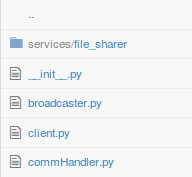
\includegraphics{figures/fstrucure}
\caption{Folder structure of cloudlet hosting ``file\_sharer" service.}
\label{fig:folderstructure}
\end{figure}

The description text file contains metadata of the services. The following is a  snippet of the description file of the file sharing service:

\begin{lstlisting}
Name=file_sharer
Description=A service for sharing files with co-located friends.
Authors=Zola Mahlaza <adeebnqo@gmail.com>
Website=http://adeebnqo.github.io/cloudlets
CloudletV=1.4
Copyright=Copyright 2014 Zola Mahlaza
\end{lstlisting}


\begin{center}
\begin{tabular}{ l | c }
  \hline                       
  Name & This is the name of the service. No spaces should be exist in the service name. \\ \hline
  Description & This is a description of the service. There is currently no maximum length. The client UI should take this into account. \\ \hline
  Authors & Creator(s) of the service. \\ \hline
  Website & Url to the web page containing more information about the service. \\ \hline
  CloudletV & Version of the cloudlet this service is compatible with. \\ \hline
  Copyright & Copyright notice. \\
  \hline  
\end{tabular}
\end{center}

All services developed for the cloudlet abide by the interface illustrated in figure \ref{fig:serviceinterface}. The start method should start the service and return, it should not block. It is suggested that one must use multiple threads.
The ``request\_service" method provides the IP the service's server socket is listening on and an open port. These values are to be returned in the form ``<IP>:<Port>".

\begin{figure}[!h]
\centering
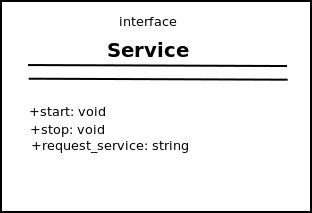
\includegraphics{figures/serviceinterface}
\caption{Interface for cloudlet services.}
\label{fig:serviceinterface}
\end{figure}

The following is an example of a service that implements the interface shown in
figure \ref{fig:serviceinterface}. It should be noted that all other non-relevant methods and local class variables are not shown.

\begin{lstlisting}
class file_sharer():
	def request_service(self):
		(host,port) = self.sockt.getsockname()
		return '{0}:{1}'.format(host,port)
	def stop(self):
		self.sockt.close()
	def start(self):
		t = threading.Thread(target=self.wait_connections)
		t.daemon = True
		t.start()
\end{lstlisting}

\subsection{Client hosted services}
Services on the mobile follow a similar approach. The difference lies how the cloudlet discovers them. Services which are located on cloudlet are loaded into execution by the service manager. However, if services are located on the client side then it is necessary for them to be advertized so that the service manager can discover them.


\section{Conclusion}
The platform at hand uses a service-oriented architecture. The base of the platform supports a limited number of actions. The capabilities of the platform can be further expanded through developed services. Communication between the cloudlet and all clients is done through the MQTT protocol. This is a lightweight machine to machine messaging protocol for use on top of the TCP/IP protocol. The services which extend the cloudlet can be physically located on the mobile device or the device that hosts the cloudlet. Figure \ref{fig:protocol} shows the physical location of services in the cloudlet. The services which extend the cloudlet need to use raw sockets. That is, they should create a server using raw sockets and not use the MQTT protocol as it has limitations in the message payload size. When a user request a service, they should be provided an ip and port. Those details will be used to communicate.

\begin{figure}[!h]
\centering
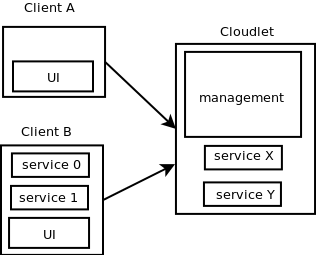
\includegraphics[scale=0.5]{figures/protocol}
\caption{Physical location of services}
\label{fig:protocol}
\end{figure}